\documentclass{beamer}
\usepackage{amsmath, amsfonts, epsfig, xspace, relsize}
\usepackage{algorithm,algorithmic, graphicx,amssymb}
\usepackage{pstricks,pst-node}
\usepackage{multimedia}
\usepackage[normal,tight,center]{subfigure}
\setlength{\subfigcapskip}{-.5em}
\usepackage{beamerthemesplit}
\usepackage{xcolor}
\usepackage{IEEEtrantools}
\newcommand{\non}{\nonumber}
\usepackage{pdfpages}
\usepackage{fancyhdr}
\usepackage{fancyvrb}
\usepackage[format=hang, font=bf]{caption}
\setbeamertemplate{caption}[numbered]
\renewcommand{\tablename}{表}
\renewcommand{\figurename}{圖}
\usepackage{fontspec}  %加這個就可以設定字體
\usepackage{xeCJK}       %讓中英文字體分開設置
\setCJKmainfont[ItalicFont=王漢宗中仿宋繁, BoldFont=標楷體]{王漢宗細圓體繁}
%\newfontfamily{\K}{BiauKai}
\setmonofont[Scale=1]{Courier New} % 等寬字型
\setsansfont[Scale=1]{Times New Roman}
%\setCJKmainfont{細明體} %設定中文為系統上的字型,而英文不去更動,使用原TeX字型
\XeTeXlinebreaklocale "zh"             %這兩行一定要加,中文才能自動換行
\XeTeXlinebreakskip = 0pt plus 1pt     %這兩行一定要加,中文才能自動換行
%\usetheme{lankton-keynote}
\usetheme{Madrid}

\author[蔡佳泓]{蔡佳泓}

%\title[Statistical Methods for Social Sciences\hspace{.1em}\insertframenumber/\inserttotalframenumber]{Probability Theory}

\title[Statistical Methods for Social Sciences]{描述統計}

\date[2017/3/7]{2017年3月7日} %leave out for today's date to be insterted

\institute[]{國立政治大學東亞所暨選舉研究中心}

\begin{document}

\maketitle
\tableofcontents
\section{Descriptive statistics}  % add these to see outline in slides

\begin{frame} \frametitle{描述統計}
  \begin{itemize}
  \item 以最有效率的方式描述人口或是特定群體的量化或類別變數的重要特徵
\item 分析單位可以是個體或是群體。
\item 群體的描述統計,例如:都市化、經濟成長率、競爭力、購買力$\ldots$
\item 個體的描述統計,例如:個人的性別、教育程度、滿意度、收入、政治態度$\ldots$
\item 可分為中央趨勢以及離散程度兩個面向
\item 可以以文字或者是圖形表示
\end{itemize}
\end{frame}
\begin{frame} \frametitle{次數分配表}
\begin{itemize}
  \item 可以用表格描述變數的分佈,例如調查中國的鄉村得到的結果,以次數分配表\ref{tab:county}表示:

  \begin{table}
  \caption{鄉村的政治型態}
\label{tab:county}
  \begin{tabular}{lrrr}
  \hline
  &次數&\% & 累積\%\\
 \hline
  村代會&52&22.22&22.22\\
  村委會&75&32.05&54.27\\
  黨支部&39&16.67&70.94\\
  聯席會議&45&19.23&90.17\\
  其他&23&9.82&100.00\\
  \hline
  總數&234&100.00\\
\end{tabular}
\end{table}
\item 可以看出相對多數的鄉村以村委會權力最大。
\item 次數與百分比都是重要的資訊,不過百分比相較起來更重要。
 \end{itemize}
\end{frame}
\begin{frame} \frametitle{直方圖}
\begin{itemize}
\item 可以用圖形表示變數的次數分配,藉以描述其特徵。
\item 適用於類別變數,可表示各類別的次數、百分比等。
\item 可找出相對多數的類別,也可以標示數值方便閱讀。
\end{itemize}
\end{frame}
\begin{frame}\framtitle{R 的直方圖}
\begin{figure}
\begin{center}
\includegraphics[scale=.5]{week3_plot1.jpg}
\end{center}
\end{figure}
\end{frame}
\begin{frame}\frametitle{R 的水平直方圖}
\begin{figure}
\begin{center}
\includegraphics[scale=0.5]{week3_plot1_1.jpg}
\end{center}
\end{figure}
\end{frame}
\begin{frame}\frametitle{R 的水平直方圖}
\begin{figure}
\begin{center}
\includegraphics[scale=0.5]{week3_plot_mode.jpg}
\end{center}
\end{figure}
\end{frame}
\begin{frame}\frametitle{Excel 直方堆疊圖}
\begin{figure}
\begin{center}
\includegraphics[scale=0.8]{stackedbarex1.png}
\end{center}
\end{figure}
\end{frame}
\begin{frame} \frametitle{長條圖}
\begin{itemize}
\item 適用於連續變數(如果太過離散則需要適當地分組)
\item 可表示變數中各個值的次數、百分比、密度等。
\item 若用於百分比,直方的高度累加=1(類似百分比的長條圖)。
\item 假設資料成一定的分佈,例如常態分佈,求出資料的平均值、離散程度等參數之後,可以加上平滑曲線。
\item 也可以用核心密度(kernel density)顯示資料的分佈,曲線下的面積=1,而直方的總面積=1。
\end{itemize}
\end{frame}
\begin{frame}\frametitle{SPSS 的長條圖}
\begin{figure}
\begin{center}
\includegraphics[scale=.45]{outhistex1.png}
\end{center}
\end{figure}
\end{frame}
\begin{frame}\frametitle{加上平滑曲線 R 的長條圖}
\begin{figure}
\begin{center}
\includegraphics[scale=.5]{week3_plot2.jpg}
\end{center}
\end{figure}
\end{frame}
\begin{frame}\frametitle{加上文字或線條標示 R 的長條圖}
\begin{figure}
\begin{center}
\includegraphics[scale=.5]{taipeicitypredict.jpg}
\end{center}
\end{figure}
\end{frame}

\begin{frame} \frametitle{餅狀圖}
\begin{itemize}
\item 適用於類別變數
\item 可表示變數中各類別的百分比
\item 為了閱讀方便,可加上百分比
\item 如果類別太多,視覺上不易比較各個類別的大小,不適合使用餅狀圖
\end{itemize}
\end{frame}
\begin{frame}\frametitle{加上數值的 Excel 餅狀圖}
\begin{figure}
\begin{center}
\includegraphics[scale=.4]{outpieex1.png}
\end{center}
\end{figure}
\end{frame}
\begin{figure}\frametitle{R 的餅狀圖}
\begin{center}
\includegraphics[scale=.5]{Week1_pie1.jpg}
\end{center}
\end{figure}
\end{frame}
\begin{frame}
\begin{figure}
\begin{center}
\includegraphics[scale=.5]{Week1_pie2.jpg}
\end{center}
\end{figure}
\end{frame}
\begin{frame} \frametitle{R 的點狀圖}
\begin{itemize}
\item 適用於類別變數
\item 可表示變數中各類別的次數,類似直方圖
\item 適用於多類別的變數
\item 可呈現按次數多寡排序後的類別
\end{itemize}
\end{frame}
\begin{frame}
\begin{figure}
\begin{center}
\includegraphics[scale=.5]{Week1_dot1.jpg}
\end{center}
\end{figure}
\end{frame}
\begin{frame}
\begin{figure}
\begin{center}
\includegraphics[scale=.5]{Week1_dot2.jpg}
\end{center}
\end{figure}
\end{frame}
\begin{frame}
\begin{itemize}\frametitle{莖葉圖}
\item 用於量化變數,可表示次數的分佈情形。
\item 莖代表至少2位數,葉代表觀察值最末一位。
\item 葉有可能自動四捨五入進位
\item 莖可能因為尺度一致而進位
\end{itemize}
\end{frame}
\begin{frame}\frametitle{範例一}
某一個系開設課程的修課人數的調查結果如下:\\
10, 12, 14, 16, 18, \\
20, 20, 20, 20, 20, 21, 21, 21, 21, 21, 22, 22, 22, 22, 22,\\
 31, 32, 33, 34, 35, 36,\\
44, 44, 45, 45, 46, 46, 47, 47, 48, 48, 49, 49, \\
50, 50\\
\bigskip
\begin{tabular}{l|l}
1&024\\
1&68\\
2&00000111112222\\
2 &\\ 
  3 & 1234\\
  3 & 56\\
  4 & 44\\
  4 & 5566778899\\
  5 & 00\\
\end{tabular}
\end{frame}
\begin{frame}\frametitle{範例二}
某鄉鎮歷年來的六月份新生兒人數的調查結果如下:\\
200 204 209 210 212 213 217 217 219 220 227 229 235 243 246 247 249 249 250 253 254 260 264 265 282 284 286 289 303 331\\
\bigskip
\begin{tabular}{l|l}
20  &049023779\\
  22 & 0795\\
  24 & 36799034\\
  26 & 045\\
  28 & 2469\\
  30 & 3\\
  32 &7 1\\
\end{tabular}
\begin{itemize}
\item 系統可能為了呈現簡潔起見,自動進位部分的數值。
\end{itemize}
\end{frame}
\begin{frame}
\begin{figure}
\begin{center}
\includegraphics[scale=.5]{week3_plot3.jpg}
\end{center}
\end{figure}
\end{frame}
\begin{frame}\frametitle{中央趨勢}
\begin{itemize}
\item 用一個統計值描述資料的分佈
\item 眾數
\item 中位數
\item 百分位數
\item 平均數
\end{itemize}
\end{frame}
\begin{frame}\frametitle{眾數}
\begin{itemize}
\item 適用於質化變數,不適用於連續變數。
\item 定義為發生最多次的那一個值。
\item 有可能超過一個。
\item 相對於其他類別,眾數所在的類別可以代表較可能發生的事件。如果知道眾數所在的類別,可以用這個類別去猜測或是代表資料以外的事件。
\item 例如已知多數的警察是男性,我們如果隨機抽出一位警察,應該會猜該受訪者是男性。但是我們仍然有 $100\times (1-m)\%$ 的機會犯錯,$m$ 代表已知警察為男性的比例,$1>m>0$。如果有其他資訊,我們可以降低 $100\times (1-m)\%$。
\item 例如已知某一個國家的警察之中有6成貪污,$m=0.6$,我們有$100\times (1-0.6)\%=40\%$誤認警察收賄的可能。
\end{itemize}
\end{frame}
\section{Median}
\begin{frame}{中位數(Median, Md)}
\begin{itemize}
\item 50\%的數比它大,50\%的數比它小。
\item 中位數可用來表示收入、房屋年齡、房屋坪數、房價,例如2016年我國工業及服務業每人每月業薪資中位數為4萬853元
\item 財政部財政資訊中心提供收入的中位數與平均數資料。營建署提供房價資料。
\end{itemize}
\end{frame}
\begin{frame}\frametitle{百分位數及中位數}
\begin{itemize}
\item 第$p$個分位數表示(100-$p$)\%的數比它大,$p$\%的數比它小。
\item 可以是實際存在的數,也可以是計算所得。
\item 有數種計算方式,根據資料的分佈而定。
\item 最簡單的是遇到偶數的(已排列)資料數列,中位數是$\frac{a+b}{2}$,$a$、$b$是 50\% 資料點相鄰的兩個數。如果是奇數的數列,就是找出分割一半的數。

\end{itemize}
\end{frame}
\begin{frame}\frametitle{百分位算法}
\begin{itemize}
\item 假設資料中有$n$個數,$i=1,\cdots,n$\\
\Large
%$p_{i}=100\cdot \frac{i-0.5}{n}$\\
\[i=\frac{np_{i}}{100}\]
\normalsize
\item 例如資料為:$X=(1, 1001, 1002, 1003)$
\item 25 百分位所在位置$=\frac{4\times 25}{100}=1$。因此 25百分位為 1。
\item 50 百分位所在位置為:$\frac{4\times 50}{100}=2$。因此 50百分位為 1001。

\end{itemize}
\end{frame}

\begin{frame}\frametitle{百分位算法}
\begin{itemize}
\item 假設資料中有$n$個數,$i=1,\cdots,n$\\
\Large
%$p_{i}=100\cdot \frac{i-0.5}{n}$\\
\[i=\frac{np_{i}}{100}+0.5\]
\normalsize
\item 例如資料為:$X=(1, 1001, 1002, 1003)$
\item 50百分位所在的位置$=\frac{4\times 50}{100}+0.5=2.5$
\item 因為2.5落在1001及1002中間,所以$0.5\times 1001+0.5\times 1002=1001.5$
\item 計算25百分位$=\frac{4\times 25}{100}+0.5=1.5$
\item 因為落在1及1001中間,所以$0.5\times 1+0.5\times 1001=751$
\item 計算75百分位$=\frac{4\times 75}{100}+0.5=3.5$
\item 因此,$0.5\times 1002+0.5\times 1003=1002.5$
\end{itemize}
\end{frame}
\begin{frame}\frametitle{中位數}
\begin{itemize}
\item 另外一種計算方式為先計算各個位數的落點,然後計算還要補足的距離:
\item 例:$y=2,3,4,7,9,10,12,12$
\item 中位數=$2\times \frac{N+1}{4}=4.5$。因為落在 7, 9 中間所以:$7+0.5\times (9-7)=8$
\item 25分位數$=1\times \frac{8+1}{4}=2.25$。因為位於 3 及 4 之間,故:$3+0.25\times (4-3)=3.25$
\item 75分位數$=0.75\times (8+1)=6.75。$ 
\item 因為第6個數是10,但是還要補10與下一個數12之間的距離為$10+0.75\times (12-10)=11.5$
\end{itemize}
\end{frame}
\begin{frame} \frametitle{R 以及 SPSS}
\begin{itemize}
\item \texttt{R} 設定了 9 種不同百分位的類型。假設我們不知道數字排列的形態,我們必須假設第 $k$ 個數字等於某種比例,例如 $\frac{k}{n}$,或者是 $\frac{k-1}{n-1}$。如果不指定,\texttt{R} 的內建類型是 7,不過比較常用的是類型 6,因此下面的範例設定 type=6。
\end{itemize}
\end{frame}
\begin{frame}[fragile=singleslide]\frametitle{比較SPSS與R的輸出}
\begin{itemize}
\item 例如有一筆34位學生的成績資料:\\
15, 22, 26, 32, 33,36, 36, 41, 42, 44,\\
44, 45, 47, 48, 61,63, 63, 65, 65, 65,\\
66, 66, 68, 69, 70,71, 74, 74, 76, 77,\\
78, 78, 79, 85
\item 分別用SPSS以及\texttt{R}計算25、50、75、90分位數:
\end{itemize}
\begin{verbatim}
> quantile(V1, c(.25,.5,.75,.9), type=6)
  25%   50%   75%   90% 
41.75 64.00 71.75 78.00 
\end{verbatim}
\begin{center}
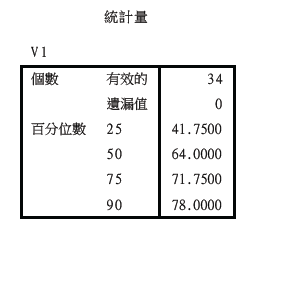
\includegraphics[scale=.65]{v1_quantile.png}
\end{center}
\end{frame}
\begin{frame}\frametitle{分組資料的中位數}
\begin{itemize}
\item 按各組的性質加以排序之後,計算中位數,視該中位數落在那一組。
\item  例如表\ref{tab:cars}顯示停車場有以下顏色的車輛:
\begin{table}
\caption{停車場的車輛顏色}
\label{tab:cars}
\begin{tabular}{| c |  c |}
\hline
Color & Frequency \\
\hline
White & 10 \\
Green & 3 \\
Yellow & 5 \\
Blue & 7 \\
Red & 4 \\
\hline
\end{tabular}
\end{table}
\item 請問中位數的汽車顏色是甚麼? 
\end{itemize}
\end{frame}
\begin{frame}\frametitle{實例}
\begin{itemize}
\item 由小而大按照數目排列車輛
\begin{table}
\begin{tabular}{| c |  c |}
\hline
Color & Frequency \\
\hline
Green & 3 \\
Red & 4 \\
Yellow & 5 \\
Blue & 7 \\
White & 10 \\
\hline
\end{tabular}
\end{table}
\item 總共有29輛汽車,中位數應該落在第15個數,所以是藍色組的汽車為中位數。
\end{itemize}
\end{frame}
\section{Mean}
\begin{frame}\frametitle{平均數}
\begin{itemize}
\item 用在量化變數或是二元變數。
\item 可以想成是觀察值的平衡點:比平均值大的數的總和等於比平均值小的數的總和的絕對值。
\item 會受到極端值的影響。
\item 可以考慮去掉頭尾的極端值再求平均數。
\item 數學上又稱為變數的第一個矩(moment)。因為變數的矩定義為:
$\mu' _{n}=\int_{-\infty}^{\infty} (x-c)^n f(x) \, \mathrm{d}x$
\item 第二個矩是變異數,也就是$\frac{1}{n}\sum (x-\bar{x})^2$,或者是$E(X^2)-E(X)^2$
\end{itemize}
\end{frame}
\begin{frame}\frametitle{平均數計算方式}
\begin{itemize}
\item $\bar{y}=\frac{\sum y}{n}$
\item $y=6, 7, 8, 8, 9, 10, 13, 15, 16, 45$
\item $\bar{y}=\frac{\sum (6+7+\cdots , +45)}{10}=13.7$
\end{itemize}
\end{frame}
\begin{frame}\frametitle{分組平均數}
\begin{itemize}
\item 計算表\ref{tab:kids}的平均數
\begin{table}
\caption{子女人數分佈}
\label{tab:kids}
\begin{tabular}{| c |  c | c |}
\hline
子女人數 (x) & 次數 (f) & xf\\
\hline
1 & 5 & 5\\
2 & 12 & 24\\
3 & 8 & 24\\
4 & 3  & 12\\
5 & 0  & 0\\
6 & 0	& 0\\
7 & 1	& 0\\
\hline
總數 & $\sum f=29$ & $\sum xf=72$\\
\hline
\end{tabular}
\end{table}
\item 平均數: $\frac{72}{29}=2.48$
\end{itemize}
\end{frame}
\begin{frame}\frametitle{分組平均數的平均}
\begin{itemize}
\item 假設觀察值分為$k=1\cdots k$個組,每一組有$y_{1}, y_{2},\cdots $ 人,每一組平均數為$\bar{y_{1}}$, $\bar{y_{2}},\cdots $,則全體的平均數為:\\
\Large
 $\bar{y}$=$\frac{\sum y_{k}\cdot \bar{y_{k}}}{n}$
 \normalsize
 \item 計算表\ref{tab:pm25}的平均數:
\begin{table}
\caption{各地$\textrm{PM}_{2.5}$濃度}
\label{tab:pm25}
\begin{tabular}{| l |  l | l | l |}
\hline
地點 &  $\textrm{PM}_{2.5}$濃度 & 個數(n)& 平均數($\bar{y_{k}}$)\\
\hline
1 & 25, 33, 44 & 3 & 34\\
2 & 43, 66, 78, 81 & 4 & 67\\
3 & 90, 76, 105, 110, 121 & 5 & 100.4\\
\hline
總數 &  & $\sum n= 12$ & $\sum n\bar{y_{k}}=102+268+$\\
  & & & $502=872$\\
\hline
\end{tabular}
\end{table}
\item $\bar{y}=\frac{872}{12}=72.66$
 \end{itemize}
\end{frame}
\section{Skewness}
\begin{frame}\frametitle{偏態}
\begin{itemize}
\item skewness
\item 測量資料是否分佈對稱
\item 正偏:右邊的尾巴較左邊長,眾數偏左
\item 負偏:左邊的尾巴較右邊長,眾數偏右
\item 常態分佈的偏態值=0
\item 樣本偏態值$=\frac{n}{(n-1)(n-2)} \frac{\sum (x_{i}-\bar{x})^3}{s^3}$
\item $s$是標準差$s=\sqrt{\frac{\sum (x-\bar{x})^2}{n}}$
\item 有偏態時須注意平均值是否會誤導。
\end{itemize}
\end{frame}

\begin{frame}\frametitle{偏態型態}
\begin{figure}
\begin{center}
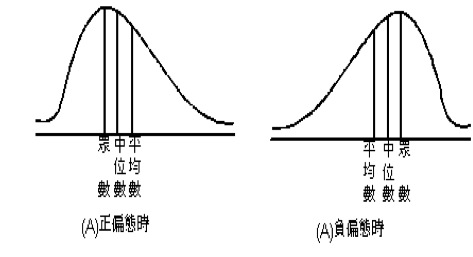
\includegraphics[scale=.6]{week3_skewness.jpg}
\end{center}
\end{figure}
\end{frame}
\begin{frame}[fragile]{比較\texttt{R}與Stata}
\begin{itemize}
\item 偏態有多種計算方式,\texttt{R}的計算公式1與2分別與Stata以及SPSS得到的結果相同。
\item 以學生的寫作成績為例:
\end{itemize}
\begin{Verbatim}[frame=single,label=\textit{R code}]
> my<-read.dta("hsb2.dta")
> attach(my)
> skewness(write, type=1)
[1] -0.4784158
\end{Verbatim}
\end{frame}
\begin{frame}{比較\texttt{R}與Stata}
\centering
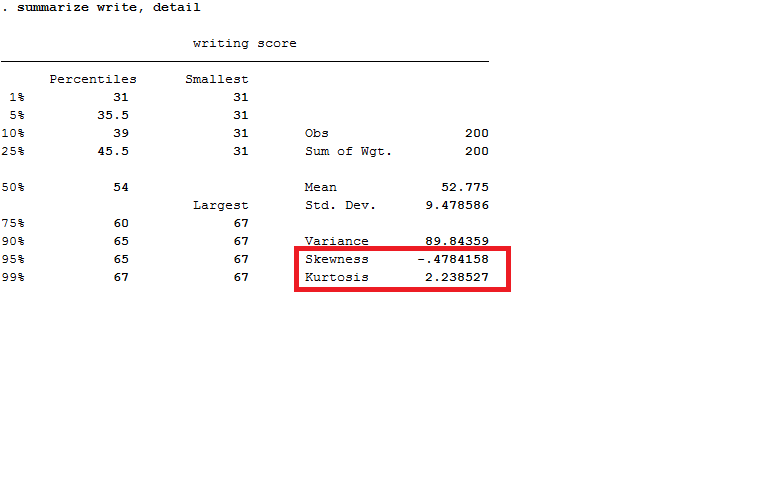
\includegraphics[scale=.8]{write_stata.png}
\end{frame}
\begin{frame}[fragile]{比較\texttt{R}與SPSS}
\begin{Verbatim}[frame=single,label=\textit{R code}]
> library(e1071)
> skewness(write, type=2)
[1] -0.4820386
\end{Verbatim}
\centering
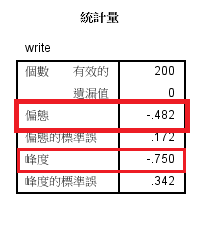
\includegraphics[scale=.8]{write_spss.png}
\end{frame}
\section{kurtosis}
\begin{frame}\frametitle{峰度}
\begin{itemize}
\item[\boxtimes] kurtosis
\item[\boxtimes] 測量資料的分佈是高聳或是平坦
\item[\boxtimes] 越平坦則兩邊尾部越長,越高聳則是靠近平均值的部份越集中
\item[\boxtimes] 偏態是第三個矩,峰度是第四個矩
\item[\boxtimes] 計算峰度的公式:
$\frac{m^4}{m^2_{2}}-3$\\
$s2=\sum (x_{i}-\bar{x})^2$\\
$s4=\sum (x_{i}-\bar{x})^4$\\
$m2=\frac{s2}{n}$
$m4=\frac{s4}{n}$\\
\item[\boxtimes] 不同統計軟體計算峰度的公式略有不同,如果用{\tt R},可以用{\tt e1071}這個包裹裡面的{\tt kurtosis},用{\tt type}指令選擇2可得到跟SPSS一樣的答案。
\item[\boxtimes] Stata的計算峰度公式為$\frac{m^4}{m^2_{2}}$
\item[\boxtimes] 樣本數目越大,理論上各種計算方式的結果越接近。
\end{itemize}
\end{frame}
\begin{frame}[fragile]{用\texttt{R}驗證Stata的峰度}
\begin{itemize}
\item 因為\texttt{R}沒有適當的計算公式得到Stata計算峰度的相同結果,使用語法計算$\frac{m^4}{m^2_{2}}$
\end{itemize}
\begin{Verbatim}[frame=single,label=\textit{R code}]
> s4=sum((my$write-mean(my$write))^4)
> s4
[1] 3577773
> m4=s4/200
> s2=sum((my$write-mean(my$write))^2)
> m2=s2/200
> (m4/m2^2)
[1] 2.238527
\end{Verbatim}
\end{frame}
\begin{frame}[fragile]{比較\texttt{R}與SPSS}
\begin{Verbatim}[frame=single,label=\textit{R code}]
> library(e1071)
> kurtosis(write, type=2)
[1] -0.7502476
\end{Verbatim}
\centering
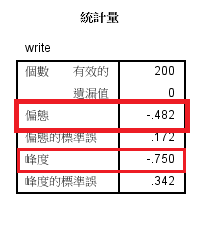
\includegraphics[scale=.8]{write_spss.png}
\end{frame}
\begin{frame}\frametitle{卡方分佈的偏態與峰度}
\begin{figure}
\begin{center}
\includegraphics[scale=.48]{week3_plot_chisq1.jpg}
\end{center}
\end{figure}
\end{frame}
\begin{frame}\frametitle{常態分佈的偏態與峰度}
\begin{figure}
\begin{center}
\includegraphics[scale=.48]{week3_plot_normal.png}
\end{center}
\end{figure}
\end{frame}
\begin{frame}\frametitle{Gamma分佈的偏態與峰度}
\begin{figure}
\begin{center}
\includegraphics[scale=.48]{week3_plot_gamma.png}
\end{center}
\end{figure}
\end{frame}
\section{deviation}
\begin{frame}\frametitle{離散}
\begin{itemize}
\item 第一種測量方式為範圍
\item 範圍(range):最大值及最小值的差距。
\item 若是常態分佈,範圍約等於六個標準差。
\item 平均數相同,範圍可能不同(A\& F, p. 46)

\end{itemize}
\end{frame}
\begin{frame}\frametitle{}
\begin{itemize}
\item 樣本變異數:母體變異數的無偏估計
\begin{equation}
\textrm{Variance}=\frac{\sum (X-\bar{X})^2}{n}
\end{equation}
\item 代表觀察值與平均數之間的差距
\item 樣本標準差為變異數的平方根
\begin{equation}
\textrm{s.d.}=\sqrt{\frac{\sum (X-\bar{X})^2}{n}}
\end{equation}
\item 如果樣本來自二元分佈,即0,1,則樣本標準差為:\\
\[\sqrt{\frac{np(1-p)}{n-1}}\]
其中 $p$ 是事件發生的機率。
\end{itemize}
\end{frame}
\begin{frame}
\begin{itemize}\frametitle{標準差}
\item 大於或等於0
\item 因為是樣本標準差,故用n-1當分母
\item 如果樣本成常態分配,利用微積分可求出平均數的$\pm$1個標準差包含約68\%的樣本。$\pm$2個標準差包含約95\%的樣本。$\pm$3個標準差包含約99\%的樣本。
\item 例如我們有一筆3000位員工薪資的資料,畫成長條圖近似常態分配。
\item 經過調整成平均值=0,標準差=1之後,一個標準差大約佔68\%的面積,兩個標準差佔95\%的面積。
\item 標準化常態分佈:$\phi(x)=f_{N}(0,1)=\frac{1}{2\pi}exp(-\frac{x^2}{2})$
\end{itemize}
\end{frame}
\begin{frame}\frametitle{長條圖}
\begin{figure}
\begin{center}
\includegraphics[scale=.48]{week3_salary1.jpg}
\end{center}
\end{figure}
\end{frame}

\begin{frame}\frametitle{常態分佈圖}
\begin{figure}
\begin{center}
\includegraphics[scale=.48]{week3_salary2.jpg}
\end{center}
\end{figure}
\end{frame}

\begin{frame}\frametitle{標準化常態分佈}
\begin{figure}
\begin{center}
\includegraphics[scale=.48]{week3_plot_normal1.jpg}
\end{center}
\end{figure}
\end{frame}
\begin{frame}\frametitle{標準化常態分佈}
\begin{figure}
\begin{center}
\includegraphics[scale=.48]{week3_plot_normal2.jpg}
\end{center}
\end{figure}
\end{frame}
\begin{frame}\frametitle{Z值或分數}
\begin{itemize}
\item 考慮母體資料中的標準差與平均值,標準化觀察值以比較觀察值與平均值之間的距離
\[z=\frac{x_{i}-\bar{x}}{\sigma}\]
\[\sigma\neq 0\]
\item 標準化常態分佈的$Z$值介於-3.4到3.4之間。
\item $Z$值可轉換為百分位,百分位也可轉換為$Z$值。標準化常態分佈的$Z$=-1.96時,由左到右端點面積為2.5\%。
\item 有一位員工的今年月薪為8.5萬,去年則為8萬,而去年的全體薪水標準差為2萬,平均值為6.5萬,今年的全體薪水標準差為2.9萬,平均值為6萬,請問該員工月薪相較於全體員工有增加嗎?
\[z_{1}=\frac{8.5-6}{2.29}=0.87\]
\[z_{2}=\frac{8-6.5}{2}=0.75\]
\item 因為$z_{1}\geq z_{2}$,因此有增加。
\end{itemize} 
\end{frame}
\begin{frame}\frametitle{例}
\begin{itemize}
\item 2009年的中國「春運」,據估計有23.2億的旅客運量。假設把所有轉車都算成一次,各大車站估計旅客人數(單位:萬)為$50, 52, 55, 28, 30, 35, 40, 49, 32, 19, 15, 61, 43,47, 44, 70, 83, 66, 88, 85, 36, 36, 47, 49,67, 68$等。
\item 計算平均值以及標準差
\item 由此可知68\%的車站的估計旅客人數落在49.8-19.38萬及49.8+19.38萬之間,也就是在30萬與70萬之間。
\end{itemize} 
\end{frame}
\begin{frame}\frametitle{}
\begin{figure}
\begin{center}
\includegraphics[scale=.48]{week3_plot_spring.jpg}
\end{center}
\end{figure}
\end{frame}
\begin{frame}\frametitle{標準差的另一種求法}
\begin{itemize}
\item 由於平均數的$\pm$三個標準差包含99.7\%的樣本,如果知道樣本的平均數跟最大值及最小值,而且樣本成常態分佈,便可以估計標準差,也就是$\frac{range}{6}$。
\item 例如,據說愛因斯坦、莫扎特智商160,一般人智商分佈在55以及145之間,平均智商為100,標準差為$\frac{145-55}{6}=15$,所以智商85到115的人約有68\%。
\end{itemize} 
\begin{figure}
\begin{center}
\includegraphics[scale=.5]{iqplot.jpg}
\end{center}
\end{figure}
\end{frame}
\begin{frame}[fragile]{標準差的特性}
\begin{itemize}
\item 改變樣本的單位,標準差也會改變
\item 例:
\begin{verbatim}
H<-c(15000,7000,19000,3000,15000,19000,4000,12000,
       17000,  9000)
\end{verbatim}
\item $\sigma_{H}=$ 5962.848
\begin{verbatim}
h<-c(15,7,19,3,15,19, 4,12,17, 9)
\end{verbatim}
\item $\sigma_{h}=$5.962
\item 加減樣本的值會改變平均值,但是不會改變標準差,因為$\sum_{i=1\sim n} (x_{i}-\bar{x})$變成$\sum ((x_{i}+k)-\overline{x+k})=\sum x_{i}+k-\frac{\sum x}{n}-\frac{nk}{n}=\sum (x_{i}-\bar{x})$
\end{itemize}
\end{frame}
\section{結論}
\begin{frame}\frametitle{結論}
\begin{enumerate}
\setbeamertemplate{enumerate item}{%
  \usebeamercolor[bg]{item projected}%
  \raisebox{-.5pt}{\colorbox{bg}{\color{fg}\footnotesize\insertenumlabel}}%
}
%\begin{equation}‎
%var(aX)‎ ‎=‎ \mathlarger{\mathlarger{‎‎\sum}}_{x}^{‎}(aX-E[aX])^2f_{x}(x)}‎‎
%\end{equation}‎
\item 認識描述統計的資料描述方式:
\begin{itemize}
\item 次數分配表
\item 直方圖
\item 長條圖
\item 餅狀圖
\item 點狀圖
\end{itemize}
\item 認識中央趨勢:
\begin{itemize}
\item 眾數
\item 中位數
\item 百分位數
\item 平均數
\end{itemize}
\item 認識偏態與峰度
\item 認識離散程度:
\begin{itemize}
\item 變異數
\item 標準差
\item $z$值
\end{itemize}
\end{enumerate}
\end{frame}
\end{document}
